\documentclass[a4paper,12pt]{article}

% Packages
\usepackage{graphicx}   % For diagrams
\usepackage{geometry}   % Page layout
\usepackage{hyperref}   % Hyperlinks
\usepackage{titlesec}   % Formatting section titles
\usepackage{enumitem}   % Bullet points
\usepackage{caption}    % Figure captions
\usepackage{tikz}       % UML diagrams
\usetikzlibrary{positioning}

% Page setup
\geometry{left=2.5cm, right=2.5cm, top=2.5cm, bottom=2.5cm}

% Title Formatting
\titleformat{\section}{\Large\bfseries}{\thesection}{1em}{}

\begin{document}

% Title
\begin{center}
    {\LARGE \textbf{HCLI - Habit Tracker CLI}}\\[0.5cm]
    {\Large \textbf{Development Phase}}\\[0.3cm]
    {\small Author: Alejandro Moral Aranda \hspace{1cm} Date: \today}
    \hrule
\end{center}

% Section: Implementation Overview
\section{Implementation Overview}
After defining the conceptual foundation in the previous phase, the HCLI (Habit Tracker CLI) has been developed following a structured approach. The main objective was to ensure a functional, efficient, and user-friendly habit tracking experience within a command-line interface.

Development focused on core functionalities, ensuring stability, data persistence, and analytics features while following the defined roadmap.

% Section: Development Process
\section{Development Process}
The implementation followed a structured plan:

- Building the CLI Framework: The application was built using the Typer library for intuitive command handling.
- Data Storage System: Habit data is stored in JSON files, allowing persistence and easy retrieval.
- Core Habit Management: Users can add habits, check them off, and delete them.
- Analytics and Insights: Features like streak tracking, habit summaries, and pending habit reminders were implemented.
- Testing and Debugging: Pytest was used to ensure the reliability of habit tracking functionalities.
- User Interaction Enhancements: Rich was integrated to improve the command-line interface with color-coded tables and summaries.

% Section: Challenges and Solutions
\section{Challenges and Solutions}
During development, various challenges were encountered and resolved:

- Handling User Input Robustly:  
  - Issue: CLI commands needed to handle missing or incorrect inputs.  
  - Solution: Implemented validation and error handling for missing arguments and incorrect formats.

- Ensuring Data Integrity:  
  - Issue: Avoiding corruption of JSON files when multiple commands modify them.  
  - Solution: Implemented safe read/write operations with exception handling.

- Managing Habit Streaks Accurately:  
  - Issue: Detecting broken and continued streaks based on habit periodicity.  
  - Solution: Developed an algorithm that dynamically calculates streaks for daily and weekly habits.

- Enhancing User Experience:  
  - Issue: Providing a more engaging CLI without a GUI.  
  - Solution: Used Rich for color-coded outputs, tables, and ASCII dashboards.

% Section: Updated System Architecture
\section{Updated System Architecture}
The implementation resulted in a well-structured system, refined from the conceptual phase. The key components are:

- Command Handler: Interprets and executes user commands.
- Data Manager: Stores and retrieves habit-related information.
- Analytics Engine: Calculates streaks, pending habits, and habit performance.
- Visualization Module: Displays data in an ASCII-based or graphical dashboard.

\begin{center}
\begin{figure}[h]
    \centering
    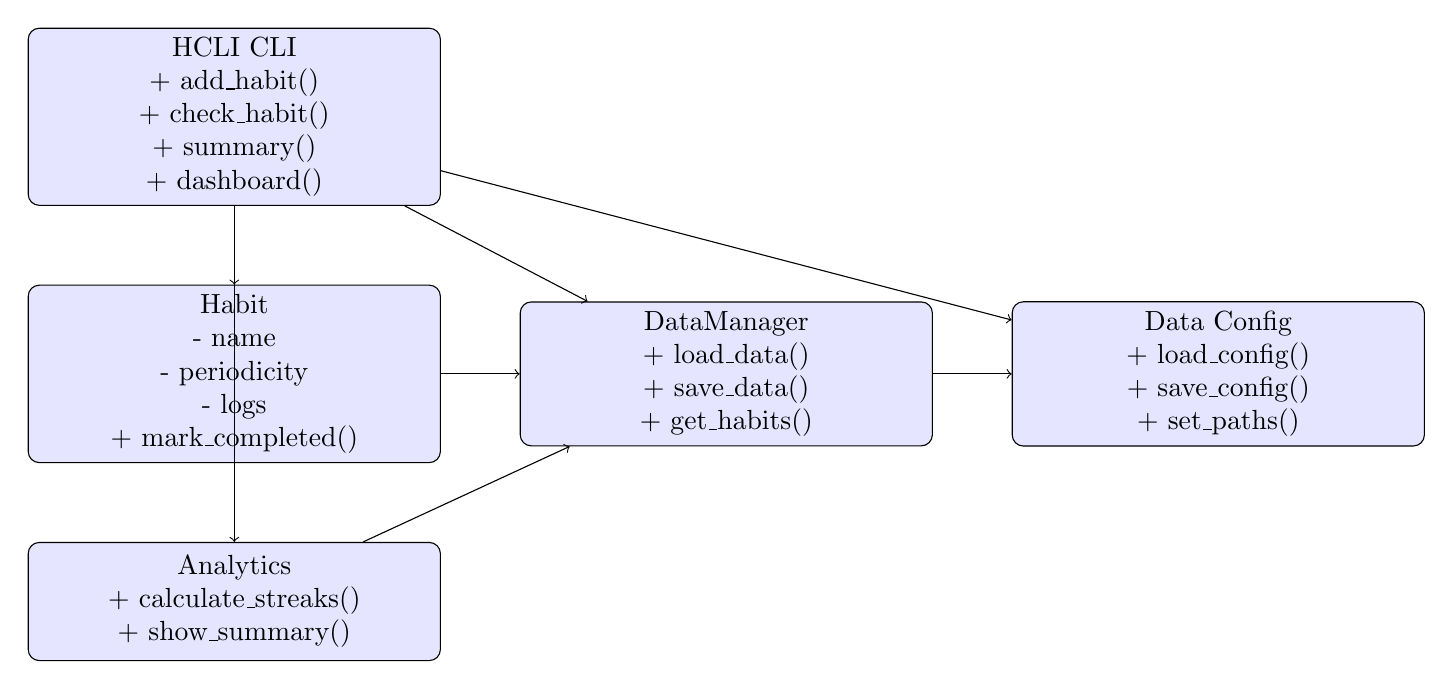
\begin{tikzpicture}[
        class/.style={rectangle, draw, fill=blue!10, rounded corners, text width=5cm, minimum height=1.5cm, align=center},
        interface/.style={rectangle, draw, fill=red!10, dashed, text width=5cm, minimum height=1.5cm, align=center}
    ]

    % Classes
    \node[class] (cli) {HCLI CLI \\ + add\_habit() \\ + check\_habit() \\ + summary() \\ + dashboard()};
    \node[class, below=of cli] (habit) {Habit \\ - name \\ - periodicity \\ - logs \\ + mark\_completed()};
    \node[class, right=of habit] (data) {DataManager \\ + load\_data() \\ + save\_data() \\ + get\_habits()};
    \node[class, below=of habit] (analytics) {Analytics \\ + calculate\_streaks() \\ + show\_summary()};
    \node[class, right=of data] (config) {Data Config \\ + load\_config() \\ + save\_config() \\ + set\_paths()};

    % Relationships
    \draw[->] (cli) -- (habit);
     \draw[->] (cli) -- (config);
    \draw[->] (cli) -- (data);
    \draw[->] (cli) -- (analytics);
    \draw[->] (habit) -- (data);
    \draw[->] (analytics) -- (data);
    \draw[->] (data) -- (config);

    \end{tikzpicture}
    \caption{Updated UML Class Diagram for HCLI with Data Config}
\end{figure}

\end{center}

% Section: Intermediate Progress
\section{Intermediate Progress}
Key milestones completed so far:

- Core functionalities fully implemented.
- Successful handling of habit storage and retrieval.
- Streak tracking and habit analytics working correctly.
- Command-line interface refined for better user interaction.
- Initial test cases running successfully with Pytest.

% Section: Next Steps
\section{Next Steps}
To finalize the implementation, the following enhancements will be made:

- Improve test coverage by expanding Pytest cases.
- Refine the dashboard visualization to provide better insights.
- Optimize data storage operations for better performance.
- Gather user feedback and implement improvements.

% Section: Conclusion
\section{Conclusion}
The development phase of HCLI has successfully transformed the initial concept into a functional CLI-based habit tracker. The system is stable, intuitive, and efficient, and will be refined further before the final submission.

\end{document}
